% ==============================================================================
% TCC - Nome do Aluno
% Capítulo 3 - Proposta do Trabalho
% ==============================================================================
\chapter{Proposta do Trabalho}
\label{sec-proposta}

Nesta seção é apresentada uma proposta para a estimativa dos parâmetros do 
modelo compartimental para dados epidemiológicos.
O modelo utilizado é apresentado, assim como a arquitetura da PINN utilizada.  
São também detalhados os testes para averiguar a efetividade do método.

\section{Estimativa de parâmetros}

Os modelos compartimentais possuem parâmetros de transmissão e mortalidade
fixos, considerando que estes modelos foram pensados apenas para dar 
uma projeção de como uma epidemia evoluirá. Entretanto, medidas de afastamento
social são capazes de alterar o parâmetro de transmissão ao longo do tempo.
Utilizando \cite{long-etal:21-L2} como inspiração, é proposto obter o parâmetro
$\beta$ como uma função em função do tempo. A rede neural deverá se ajustar 
a um $\beta(t)$. O modelo \textit{SIR} passa a ser escrito como, 

\begin{eqnarray}
   \frac{dS(t)}{dt} &=& -\frac{\beta(t) S(t)}{N} I(t),  \quad t > t_0, \label{eq:SIR-beta-t-1}\\
   \frac{dI(t)}{dt} &=& \frac{\beta(t) S(t)}{N} I(t) - \gamma I(t), \quad t > t_0, \label{eq:SIR-beta-t-2}\\
   \frac{dR(t)}{dt} &=& \gamma I(t),  \quad t > t_0, \label{eq:SIR-beta-t-3}
\end{eqnarray}

A taxa de mortalidade de um doença permanece a mesma para a maioria das doenças,
logo não há a necessidade de transformá-lo numa equação em função do tempo.
Considerando esse fato e seguindo o que foi aplicado em trabalhos como 
\cite{millevoi-etal:24-split-join-pinns} e \cite{ouyoussef-etal:24-subcompartimentos}, 
pode-se simplificar o sistama de equações acima, considerando que 
$S(t) + I(t) + R(t) = N$ para todo $t > t_0$.
A função $R(t)$ passa então a ser obtida pela subtração do total de individuos
na população pelos valores de $S(t)$ e $I(t)$.  

\begin{equation} \label{eq:Rt}
   R(t) = N - S(t) - I(t)
\end{equation}

A rede neural passar a ter que aproximar uma função $R \rightarrow R^3$ de 
$(S, I, \beta)$ em função de $t$ como ilustrado 
na figura \ref{fig:arquitetura-rede-solucao}.

\begin{figure}[htpb]
\centering
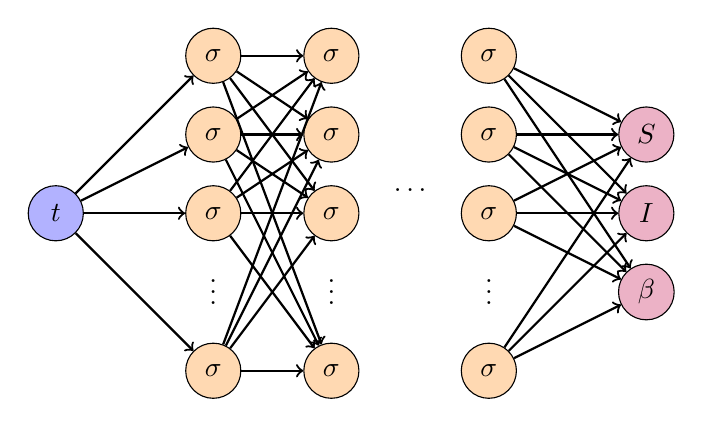
\begin{tikzpicture}[
    neuron/.style={circle, draw, minimum size=0.7cm},
    layer/.style={rectangle, minimum width=1.5cm, minimum height=8cm, draw=black, fill=blue!10, rounded corners=3pt},
    input/.style={neuron, fill=blue!30},
    hidden/.style={neuron, fill=orange!30},
    output/.style={neuron, fill=purple!30},
    physnode/.style={rectangle, draw, rounded corners, fill=orange!30, minimum width=1.5cm, minimum height=1.8cm},
    lossnode/.style={rectangle, draw, rounded corners, fill=yellow!30, minimum width=2cm, minimum height=3.2cm, align=center},
    every edge/.style={draw, ->, thick}
]

\node[input] (I-1) at (0, 2) {$t$};

\node[hidden] (H1-1) at (2, 4) {$\sigma$};
\node[hidden] (H1-2) at (2, 3) {$\sigma$};
\node[hidden] (H1-3) at (2, 2) {$\sigma$};
\node at (2, 1.1) {$\vdots$};
\node[hidden] (H1-4) at (2, 0) {$\sigma$};

\node[hidden] (H2-1) at (3.5, 4) {$\sigma$};
\node[hidden] (H2-2) at (3.5, 3) {$\sigma$};
\node[hidden] (H2-3) at (3.5, 2) {$\sigma$};
\node at (3.5, 1.1) {$\vdots$};
\node[hidden] (H2-4) at (3.5, 0) {$\sigma$};

\node at (4.5, 2.3) {$\dots$};

\node[hidden] (Hn-1) at (5.5, 4) {$\sigma$};
\node[hidden] (Hn-2) at (5.5, 3) {$\sigma$};
\node[hidden] (Hn-3) at (5.5, 2) {$\sigma$};
\node at (5.5, 1.1) {$\vdots$};
\node[hidden] (Hn-4) at (5.5, 0) {$\sigma$};

\node[output] (O-1) at (7.5, 3) {$S$};
\node[output] (O-2) at (7.5, 2) {$I$};
\node[output] (O-3) at (7.5, 1) {$\beta$};

% Connections

\foreach \j in {1,...,4}
    \path (I-1) edge (H1-\j);

\foreach \i in {1,...,4}
    \foreach \j in {1,...,4}
        \path (H1-\i) edge (H2-\j);

\foreach \i in {1,...,4}
    \foreach \j in {1,...,3}
        \path (Hn-\i) edge (O-\j);

\end{tikzpicture}
\caption{Representação gráfica das redes \textit{feedfoward}. Fonte: elaborada pelos autores.}
\label{fig:arquitetura-rede-solucao}
\end{figure}

\section{Testes com Dados Sintéticos}

Para averiguar se o método proposto funcionará bem com dados reais,
será feito primeiramente um teste com dados sintéticos obtidos a patir da solução
do modelo compartimental utilizando o método de Runge-Kutta de 4º ordem (RK4)
implementado na biblioteca \textit{SciPy} \cite{scipy}. O método resolverá 
o sistema de equações diferencias ao aproximar funções para os 3 compartimentos
do modelo \text{SIR} com o parãmetro $\beta$ em função do tempo. O único que 
será conhecido previamente, será justamente a função que descreve $\beta$.
Para emular um beta que varia em função do tempo, 
a função \ref{eq:beta_t_sintetetico} será utilizada,

\begin{equation} \label{eq:beta_t_sintetetico}
    \beta(t) = \sin(\frac{2\pi t}{t_f - t_0})  + \beta_{min}
\end{equation}

\begin{figure}[htpb]
\centering
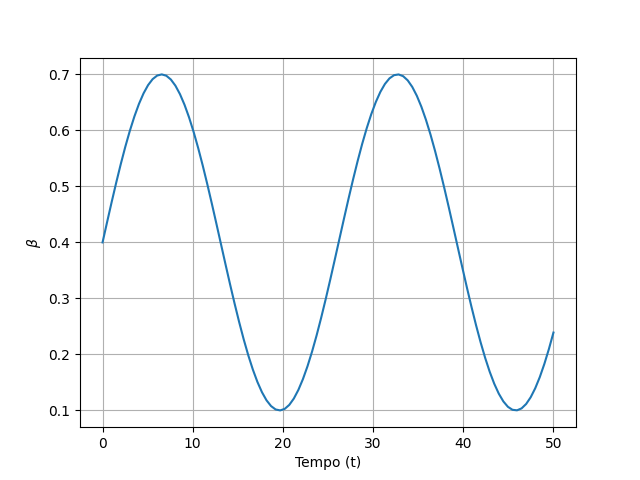
\includegraphics[width=0.6\textwidth]{figuras/real-beta-sir-nonoise.png}
\caption{Na primeira. Fonte: elaborada pelos autores.}
\label{fig:beta-sir-semruido}
\end{figure}

O modelo empregado é ligeiramente diferente do \textit{SIR} original. 
Será utilizada a sua forma normalizada, bastando remover o divisor $N$
das equações,

\begin{eqnarray}
   \frac{dS(t)}{dt} &=& -\beta(t) S(t) I(t),  \quad t > t_0, \label{eq:SIR-beta-t-1-norm}\\
   \frac{dI(t)}{dt} &=& \beta(t) S(t) I(t) - \gamma I(t), \quad t > t_0, \label{eq:SIR-beta-t-2-norm}\\
   \frac{dR(t)}{dt} &=& \gamma I(t),  \quad t > t_0, \label{eq:SIR-beta-t-3-norm}
\end{eqnarray}

Os compartimentos do modelo passam a ter um outro significado, não mostrado
mais o número de indivíduos em cada compartimento, mas sim a porcentagem 
da população que está em cada compartimento no instante $t$. 
Logo, a soma dos três compartimentos será igual a $1$ para todo instante $t$

\begin{equation}
    S(t) + I(t) + R(t) = 1, \quad t > t_0
\end{equation}

Levando isso em conta, as condições iniciais do problema são também expressadas
como porcentagens.

\begin{eqnarray}
   S_0 &=& 0.99 \label{eq:S0}\\
   I_0 &=& 0.01, \label{eq:I0}\\
   R_0 &=& 0 \label{eq:R0}
\end{eqnarray}

O problema é então resolvido para $t_0 \le t \ge t_f$, sendo $t_0=0$ e $t_f=50$.
A solução númerica obtida é então utilizada para obter um conjunto de 
$N_{data}$ valores para cada compartimento do modelo \textit{SIR}. 
Para este experimento, foram usados $100$ A figura \ref{fig:dados-semruido} 

\begin{figure}[htpb]
\centering
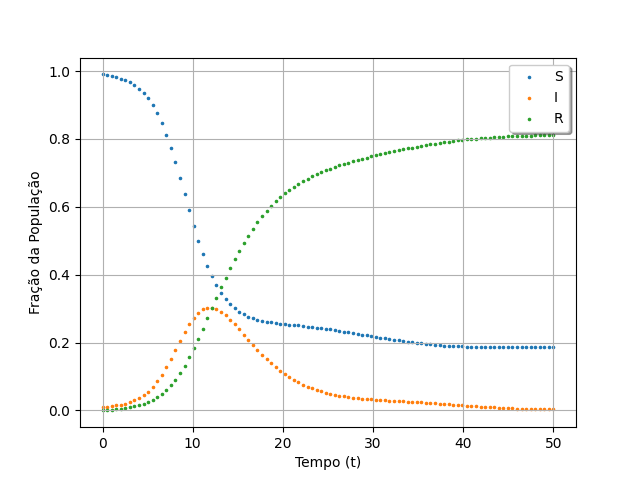
\includegraphics[width=0.6\textwidth]{figuras/runge-kutta-compartiments-data-sir-nonoise.png}
\caption{Na primeira. Fonte: elaborada pelos autores.}
\label{fig:dados-semruido}
\end{figure}

A solução com RK4 retorna dados para os três compartimentos, mas como a versão
do \textit{SIR} utilizada neste trabalho não possui a terceira equação, os 
dados para o terceiro compartimento (R) não são usados. Tomando como exemplo
trabalhos como \cite{han-etal:24-prim-artigo-alemanha} que utilizam apenas
dados do compartimento de infectados, mas conseguem bons resultados, o modelo
também será treinado apenas com dados sintéticos de incidência de infectados.  

\subsection{Avaliação dos Resultados}

A qualidade da solução obtida pela rede neural é medida pelo uso das métricas
de \textit{MSE}, norma euclidiana ($\mathcal{L}_2$) e norma no infinito 
($\mathcal{L}_{\infty}$). 
O \textit{MSE}, é definida pela equação \ref{eq:mse-metric}  

\begin{equation}\label{eq:mse-metric}
    \text{MSE} = \frac{1}{n} \sum_{i=1}^{n} (y_i - \hat{y}_i)^2
\end{equation}

A norma $\mathcal{L}_2$, é definida pela equação \ref{eq:l-2} e corresponde
a distância euclidiana entre as superfícies. È uma grandeza escalar  

\begin{equation}\label{eq:l-2}
    \mathcal{L}_2(\mathbf{x}, \mathbf{y}) = \|\mathbf{x} - \mathbf{y}\|_2 = \sqrt{\sum_{i=1}^{n} (x_i - y_i)^2}
\end{equation}

A norma $\mathcal{L}_{\infty}$, também chamada de norma máxima, é definida 
pela equação \ref{eq:l-infinity} e corresponde à distância máxima entre as
superfícies $\mathbf{x}$ e $\mathbf{y}$. A vantagem dessa métrica é mostrar
qual é o maior erro pontual. Uma desvantagem desta méstrica, é ser sensível 
a \textit{outliers}.

\begin{equation}\label{eq:l-infinity}
    \mathcal{L}_\infty(\mathbf{x}, \mathbf{y}) = \|\mathbf{x} - \mathbf{y}\|_\infty = \max_{i} |x_i - y_i|
\end{equation}

A comparação é feita com a solução númerica obtida com RK4 no caso dos 
compartimentos de sucetíveis e infectados. Para o parâmetro de taxa de infecção
$\beta$, a comparação é feita com a equação \ref{eq:beta_t_sintetetico}.

\section{Testes com Dados Sintéticos Ruidosos}

Segundo \cite{raissi-etal:19}, PINNs são resilientes a dados ruidosos. Para
testar se PINNs são capazes de corretamente aproximar as curvas do \textit{SIR}
mesmo com dados ruidosos,
é adicionado ruído gaussiano branco aos dados obtidos na seção anteior.
A equação \ref{eq:ruido-gaussiano} descreve este processo.

\begin{eqnarray}\label{eq:ruido-gaussiano}
    Z_t \sim \mathcal{N}(0, \sigma) \\
    \mathcal{N}_t = \max(\mathcal{C}_t + Z_t, 0)  
\end{eqnarray}

A figura \ref{fig:dados-comruido} mostra o resultado deste processo sobre os dados
de treinamento. Vale observar que para evitar usar dados negativos, pois são valores
que não fazem sentido no contexto do modelo, foi utilizada a função de máximo
entre o valor do dado de treinamento e zero.
Com este experimento, espera-se validar o método para a aplicação com dados reais,
que normalmente são pertubados. 

\begin{figure}[htpb]
\centering
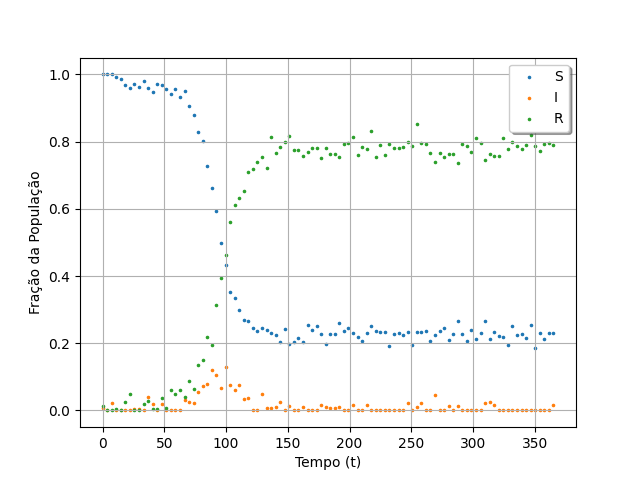
\includegraphics[width=0.6\textwidth]{figuras/runge-kutta-compartiments-data-sir-noisy.png}
\caption{Na primeira. Fonte: elaborada pelos autores.}
\label{fig:dados-comruido}
\end{figure}


\section{Testes com Base de Dados Reais}

Os dados foram coletados do plataforma \textit{OpenDataSUS} \cite{opendatasus}


\subsection{Bases de dados do DataSUS}

\subsection{Tratamento dos Dados}

\begin{figure}[htpb]
\centering
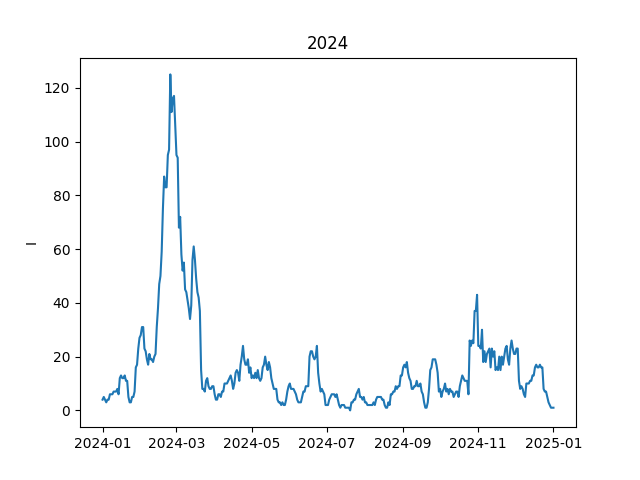
\includegraphics[width=0.6\textwidth]{figuras/data-2024-ES.png}
\caption{Na primeira. Fonte: elaborada pelos autores.}
\label{fig:dados-reais-sus-crus}
\end{figure}

Janela móvel de 7 dias como em \cite{han-etal:24-prim-artigo-alemanha},
\cite{long-etal:21-L2} e \cite{shamsara-etal:25-omicron} para suavizar o ruído


\begin{figure}[htpb]
\centering
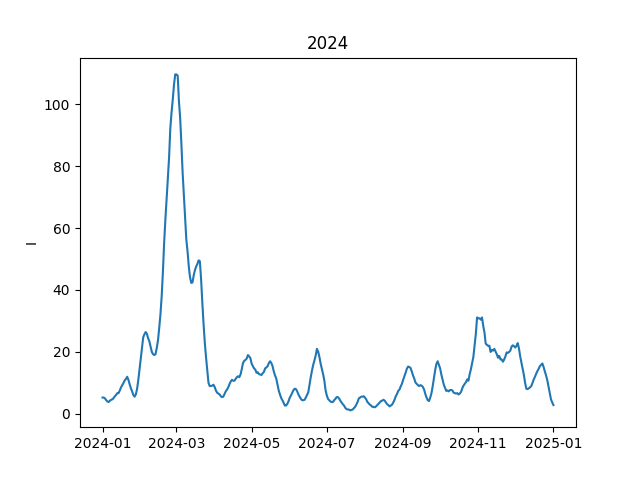
\includegraphics[width=0.6\textwidth]{figuras/smoothed-data-2024-ES.png}
\caption{Na primeira. Fonte: elaborada pelos autores.}
\label{fig:dados-reais-sus-media-movel}
\end{figure}

Pesos ajustáveis entre a loss física e a loss dos dados como em 
\cite{long-etal:21-L2} e 
\cite{shamsara-etal:25-omicron}

Segundo \cite{bonfanti-etal:24-generalizacao-pinns}, PINNs não generalizam bem
fora do domínio de treinamento. PINNs podem estimar os parâmetros para fora
do domínio de treinamento como em \cite{millevoi-etal:24-split-join-pinns}.

Assim como em \cite{ghosh-etal:23-subnotificacao}, fazer testes com lacunas
nos dados para testar a resiliência do método.

\subsection{Arquitetura da Rede}

Baseando-se em \cite{shaier-etal:22-dinns}, o número de camadas escolhido foi...

Como em \cite{millevoi-etal:24-split-join-pinns}, aplicar uma 
\textit{hard-constraint} na rede neural ao utilizar nos nós de saída
uma função de ativação que retorna apenas valores positivos.

\subsection{Parâmetro  Ajustável}

Aplicando a ideia de \cite{shamsara-etal:25-omicron}, é adicionado uma parâmetros
$\omega_{\text{dados}}$ ajustável. 

\begin{equation}\label{eq:lambda-aprendivel}
    \omega_{\text{dados}} = \frac{max(\text{gradientes de }\mathcal{L}_{\text{física}})}{\text{média}(\text{gradientes de }\mathcal{L}_{\text{dados}})}
\end{equation}

\subsection{Correlação com a Temperatura}

A gripe é uma doença com maior taxa de transmissão nos meses frios. 
Para testar se a transmissão em função do tempo aproximada pelo modelo é plausível,
é feito um teste de correlação de \textit{Pearson} entre $\beta(t)$ e a temperatura
ao longo do ano.

\subsubsection{Teste de Correlação de Pearson}

Sendo $\beta$ e $T$ duas amostras de tamanho $n$ com dados pareados $(\beta_i, T_i)$:
\begin{equation}\label{correlacao-de-pearson}
\rho = \frac{\sum_{i=1}^{n} (\beta_i - \bar{\beta})(T_i - \bar{T})}{\sqrt{\sum_{i=1}^{n} (\beta_i - \bar{\beta})^2 \sum_{i=1}^{n} (T_i - \bar{T})^2}}
\end{equation}

Espera-se um valor de $\rho$ acima de 0.5 para indicar um correlação no minímo moderada
entre a taxa de transmissão $\beta$ e a temperatura.

\subsubsection{Teste de Correlação de Spearman}

A correlação de Spearman é equivalent a calcular a correlação de Pearson nos 
\textit{ranks} dos valores.

\begin{equation}
r_s = \frac{\sum_{i=1}^{n} (R(\beta_i) - \bar{R_{\beta}})(R(T_i) - \bar{R_{T}})}{\sqrt{\sum_{i=1}^{n} (R(\beta_i) - \bar{R_{\beta}})^2 \sum_{i=1}^{n} (R(T_i) - \bar{R_T})^2}}
\end{equation}

Caso haja empates entre os elementos das amostras, aplica-se a fórmula de ajuste
abaixo.

\begin{equation}
r_s = \frac{\sum_{i=1}^{n} (R(\beta_i) - \bar{R_{\beta}})(R(T_i) - \bar{R_y})}{\sqrt{\left[\sum_{i=1}^{n} (R(x_i) - \bar{R_x})^2 - T_x\right]\left[\sum_{i=1}^{n} (R(y_i) - \bar{R_y})^2 - T_y\right]}}
\end{equation}

Sendo que os fatores $T_x$ e $T_y$ de correção de empate são calculados
usando as fórmulas abaixo.  

\begin{equation}
\mathcal{T} = \sum \frac{t^3 - t}{12}
\end{equation}


\section{Implementação}

A implementação foi feita utilizando a biblioteca \textit{DeepXDE} \cite{lu-etal:21-deepxde}, 
utilizando o \textit{TensorFlow} \cite{tensorflow:16} como \textit{backend}. 
Todo o código, dados utilizados nos experimentos,
encontram-se disponíveis no repositório público no 
GitHub\footnote{\url{https://github.com/ginbar/inverse-cm}}.
As sementes para a geração de pseudonúmeros foram fixadas para garantir
a reproducibilidade dos experimentos.
